\documentclass[../main.tex]{subfiles}
\begin{document}

\chapter{Design} \label{Chap:Design}

\section{Batteri}

\subsection{Designovervejelser}


\subsubsection{Tilgængeligt strøm}




\subsection{Beregninger}
\subsubsection{Tilgængelig strøm}


\begin{align*}
    30600s &= k \cdot 60mA + o \\
    5760s &= k \cdot 250mA + o \\
    \rightarrow k &= -130.74 \frac{s}{mA}, o = 38.44\cdot 10^3s\\
    \rightarrow T_{serviceliv} &= -130.74\frac{s}{mA} \cdot I_{drain} + 38.44\cdot 10^3s
\end{align*}


 \begin{figure}[H]
    \centering
    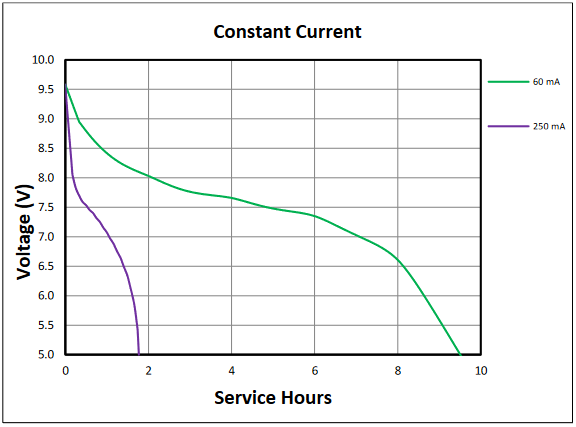
\includegraphics[scale=0.8]{Pictures/Grafer/Stroemogspaendingskurve.png}
    \captionsetup{format=hang}
    \caption{9V 6LR61 batteri duracell: spænding som funktion af tid ved konstant strømdræn\footref{fnlabel1}}
    \label{fig: batstrømkurve}
\end{figure}



\subsection{Test}

\section{Spoledesign}
\subsection{Designovervejelser}


\subsection{Beregninger}

\subsubsection{Transmitterspole/TX-spole}



\end{document}